\paragraph{}El usuario asesor puede realizar consultas sobre las reuniones,
sobre las plantillas de entrevistas de asesor que le pertenezcan y sobre su
propia información personal que exista en el sistema.
\textit{Además también puede realizar consultar de datos históricos referentes a
esta misma información en diferentes cursos académicos}.

\paragraph{}La figura \ref{diagramaNivel3-ExplotacionSistema-asesores}
muestra el nivel de abstracción 3: Explotación del sistema (módulo Asesores).

  \begin{figure}[!ht]
    \begin{center}
      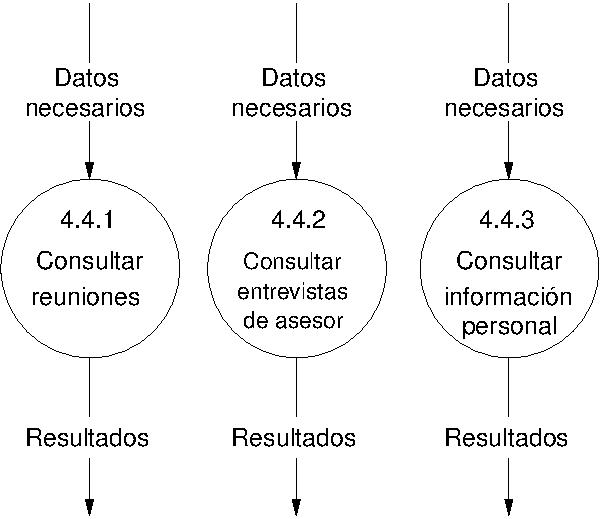
\includegraphics[]{08.Analisis_Funcional/8.2.DFDs/Niveles/Nivel3/Asesores/ExplotacionSistema/Diagramas/nivel3-ExplotacionSistema.pdf}
      \caption{Nivel de abstracción 3: Explotación del sistema (módulo Asesores).}
      \label{diagramaNivel3-ExplotacionSistema-asesores}
    \end{center}
  \end{figure}
